\section{Screening Results}\label{sec:attribution}
The screening asks which perturbations free each rest state, by which class of mechanism, and whether a matched surrogate can be told apart from force-coupled ORCA. Table~\ref{tab:matched} lists the matched pairs.
% generated by experiments/tables/make_tables45.py from paper/registry/*.yaml macros; do not edit
\begin{table}[t]
\caption{Matched surrogates against force-coupled ORCA: freed fraction at the horizon $T$ and the paired difference.}
\label{tab:matched}
\centering\scriptsize\setlength{\tabcolsep}{2pt}
\begin{tabular*}{\textwidth}{@{\extracolsep{\fill}}llcc@{}}
\toprule
Set & Perturbation & Freed & $\Delta$ [95\%] \\
\midrule
Lone keystones (\EtwoNLK{}, 120\,s) & noise $\sigma=0.07$\,m/s, 5 seeds & \EtwoLKNoiseCFreed{}/\EtwoLKNoiseCN{} & $\RvAfiveLoneEtwoDiff{}$ [$\RvAfiveLoneEtwoDiffLo{}$, $\RvAfiveLoneEtwoDiffHi{}$] \\
 & noise $\sigma=\RunNOneSigma{}$\,m/s, 20 seeds & \RunNOneFreed{}/\RunNOneRunsN{} & $\RvAfiveLoneNoneDiff{}$ [$\RvAfiveLoneNoneDiffLo{}$, $\RvAfiveLoneNoneDiffHi{}$] \\
 & force-coupled ORCA & \EtwoLKCThreeRVOFreed{}/\EtwoLKCThreeRVON{} &  \\
\addlinespace[2pt]
Second traps (\RevAsixSTSnaps{}, 120\,s) & noise $\sigma=0.07$\,m/s, 5 seeds & \RevAsixSTNoiseFreed{}/\RevAsixSTNoiseN{} & $\RvAfiveSecondEtwoDiff{}$ [$\RvAfiveSecondEtwoDiffLo{}$, $\RvAfiveSecondEtwoDiffHi{}$] \\
 & force-coupled ORCA & \RevAsixSTOrcaFreed{}/\RevAsixSTOrcaN{} &  \\
\addlinespace[2pt]
Whole runs (\EsixN{}, 600\,s) & noise $\sigma^\ast=\EsixSigmaStar{}$\,m/s & \EsixNoiseK{}/\EsixN{} & $\RvAfiveWholeDiff{}$ [$\RvAfiveWholeDiffLo{}$, $\RvAfiveWholeDiffHi{}$] \\
 & force-coupled ORCA & \EsixCThreeK{}/\EsixN{} &  \\
\addlinespace[2pt]
Pair standoffs, legacy (\PairN{}, 120\,s) & bias $+b^\ast=\PscrPairBstarPub{}$ & \PairBsPubFreed{}/\PairN{} & $\RvAfivePairLegacyDiff{}$ [$\RvAfivePairLegacyDiffLo{}$, $\RvAfivePairLegacyDiffHi{}$] \\
 & force-coupled ORCA (legacy) & \PairPubFreed{}/\PairN{} &  \\
\addlinespace[2pt]
Pair standoffs, RVO2 (\PairN{}, 120\,s) & bias $+b^\ast=\PairBstarRvo{}$ & \PairBsRvoFreed{}/\PairN{} & $\RvAfivePairRvoDiff{}$ [$\RvAfivePairRvoDiffLo{}$, $\RvAfivePairRvoDiffHi{}$] \\
 & force-coupled ORCA & \PairRvoFreed{}/\PairN{} &  \\
\bottomrule
\end{tabular*}
\par\smallskip
\parbox{\textwidth}{\scriptsize Set: number of snapshots or runs and horizon $T$. Freed: noise quenches freed by $T$ (snapshots times seeds), snapshots freed (force-coupled ORCA, bias), runs completed (whole runs). $\Delta$: freed fraction of the surrogate minus that of force-coupled ORCA, with its unadjusted 95\% interval.}
\end{table}


\subsection{Lone Keystones and Second Traps}\label{sec:att-lone}
\subsubsection{Drive and Constraint Parts.}
At the \EtwoNLK\ lone keystones force-coupled ORCA frees \EtwoLKCThreeRVOFreed\ with either solver. With the RVO2 solver its replays change no outcome (\TabThreeLKRvoReplayDis\ of \TabThreeLKRvoReplays), and its time-step response is flat ($|\ell|\le\EthreeCThreeLnRatioMax$ per snapshot). The drive part alone frees the same lone keystones. The SFM with $\tau'$ (Eq.~\eqref{eq:identity}), quenched from each snapshot, frees the same \RevAoneLoneFreed\ of \RevAoneLoneN\ lone keystones as the drive part, and \RevAoneSecondFreed\ of \RevAoneSecondN\ second traps (discordant \RevAoneDiscA:\RevAoneDiscB). The constraint part alone frees \EtwoLKConstrRVOFreed\ (RVO2) and \EtwoLKConstrPubFreed\ (legacy). The push towards the door frees \EtwoLKFrozenPlusFreed\ lone keystones, though it frees earlier than force-coupled ORCA ($\Delta$RMST $\RevAsevenPushLoneTimeEff$\,s, Holm $p\RevAsevenPushLoneTimePHolmRel$); the push away frees \EtwoLKFrozenMinusFreed. SFM and SFM+TTC free none of the screening set; TTC exerts no force at rest. The stuck-alone margin with the rest drive of force-coupled ORCA predicts which blockers force-coupled ORCA holds, with area \EtwoLKMarginAUC\ under the receiver-operating-characteristic (ROC) curve: where this margin stays positive the blocker is held, with two exceptions (\PthreeRocFreedPos\ of the \RwSixRocFreed\ freed blockers have a positive margin), and elsewhere the larger rest drive removes the rest state.

\subsubsection{Replacing the Drive.}
The stuck-alone criterion, with a coupling's rest drive in place of $mv_{\rm eff}/\tau$, predicts which blockers it frees. In couplings R1 and R2 the ORCA force (RVO2) replaces the drive instead of adding to it, with preferred velocity $v_{{\rm eff},i}\hat{\mathbf e}_i$ or $v_{0,i}\hat{\mathbf e}_i$; their rest drive is close to that of SFM. The criterion predicted before the runs that both free \RzTonezeroLoneFreed\ of the \RzTonezeroLoneN\ lone keystones, and both free exactly that one, against \RzTonezeroLoneOrcaFreed\ of \RzTonezeroLoneN\ for force-coupled ORCA, its drive part and the SFM with $\tau'$. Over the \RzTonezeroScreenN\ screening-set snapshots \RzTonezeroScreenDisagree\ outcome disagrees with the criterion, at a second trap. At the other \RzTonezeroOtherN\ second traps \RzTonezeroOtherDisagree\ disagree: \RzTonezeroOtherFreed\ are freed against \RzTonezeroOtherPredFreed\ predicted. Of the \RzTonezeroOtherHeldFreed\ predicted held and freed, \RzTonezeroOtherNeigh\ are freed after a neighbour leaves first, \RzTonezeroOtherSmall\ have margins of \RzTonezeroOtherSmallMin--\RzTonezeroOtherSmallMax\,N and \RzTonezeroOtherUnexpl\ are unexplained. The static criterion is exact for a lone blocker and incomplete once neighbours move. In whole runs (Table~\ref{tab:runsets}) R1 and R2 each complete \RzToneoneK\ of \RzToneoneN\ runs (upper bound \RzToneoneHi), against \RzToneoneRvoK\ for force-coupled ORCA on the same seeds. All \RzToneoneMoving\ still move at 600\,s: the replaced coupling evacuates slowly, which is not a deadlock.

\subsubsection{Matched Noise.}
Per-step noise at $\sigma=0.07$\,m/s (five seeds per snapshot) and at $\sigma=\RunNOneSigma$\,m/s (20 seeds) is matched to force-coupled ORCA at $T=120$\,s (Table~\ref{tab:matched}; Holm $p\RevAsevenLoneEtwoFreedPHolmRel$ and $p\RevAsevenLoneNoneFreedPHolmRel$). The level \RunNOneSigma\,m/s inverts a logit fit of the freed fraction at $\sigma=0.03$, 0.05 and 0.07\,m/s at force-coupled ORCA's \RzTonezeroLoneOrcaFreed\ of \RzTonezeroLoneN. Fitted on random halves, this rule misses the held-out half by a median \RzTfiveHeldoutMed\ [\RzTfiveHeldoutLo, \RzTfiveHeldoutHi] in freed fraction; the rule that sets $\sigma^\ast$ for whole runs misses by \RzTfiveWholeMed\ [\RzTfiveWholeLo, \RzTfiveWholeHi]. At $\sigma=0.07$\,m/s, $\beta$ from the energy span has median \PthreeBetaSevenSpanMed\ (quartiles \PthreeBetaSevenSpanQone\ and \PthreeBetaSevenSpanQthree) and lies below 1 for \RxBetaSevenSpanBelowOne\ of the \LoneBarN\ barrier-set snapshots, so this noise acts by fluctuations. From $T=\RvAfiveLoneEtwoWinFrom$ and \RvAfiveLoneNoneWinFrom\,s on, the 90\% intervals of the difference, [$\RvAfiveLoneEtwoDiffLoNinety$, $\RvAfiveLoneEtwoDiffHiNinety$] and [$\RvAfiveLoneNoneDiffLoNinety$, $\RvAfiveLoneNoneDiffHiNinety$], lie inside the margin $\pm\RvAfiveMargin$. Overlap cannot separate noise from force-coupled ORCA: two halves of the noise seeds overlap ($\Omega=\RunNOneJNoiseNoise$) as much as noise and force-coupled ORCA do ($\Omega=\RevAnineLKNHalfJ$, against \PscrLKNHalfEJ\ for independent sets, $p\RevAnineLKNHalfPRel$).

Noise frees later. Its restricted mean time to free exceeds that of force-coupled ORCA by $\PscrTimeLoneEtwoEff$\,s [$\PscrTimeLoneEtwoLo$, $\PscrTimeLoneEtwoHi$] with five seeds (Holm $p\RevAsevenLoneEtwoTimePHolmRel$) and $\PscrTimeLoneNoneEff$\,s [$\PscrTimeLoneNoneLo$, $\PscrTimeLoneNoneHi$] with 20 ($p\RevAsevenLoneNoneTimePHolmRel$). Replay separates the two by construction. With the noise stream fixed, \RvAtenFlips\ of \RvAtenNPairs\ quenches change. Across seeds noise disagrees at \TabThreeLKNoiseDisagree\ of \TabThreeLKNoiseSnaps\ snapshots with five seeds and \RevAsevenLoneNoneReplayDiscA\ of \EtwoNLK\ with 20; force-coupled ORCA replays change none.

The time step separates per-step noise as well (Fig.~\ref{fig:escape}c). With $\sigma$ set per snapshot for $\beta_0=1.5$ and 2.5 (time-step set), the escape rate rises as $\Delta t$ falls, more at $\beta_0=2.5$, as the per-step temperature of Eq.~\eqref{eq:teff} predicts. At $\beta_0=1.5$ the pooled $\ell$ is \RzTfourOnepfiveObs\ [\RzTfourOnepfiveLo, \RzTfourOnepfiveHi], against \RzTfourOnepfiveA\ from Eq.~\eqref{eq:ell} with the saddle height. At $\beta_0=2.5$ it is \RzTfourTwopfiveObs\ [\RzTfourTwopfiveLo, \RzTfourTwopfiveHi], below the saddle prediction \RzTfourTwopfiveA. Eq.~\eqref{eq:ell} assumes an Arrhenius slope of $\Delta U$. With the energy span scaled by the measured slope ratio \RzTtwoRatio\ (Sect.~\ref{sec:escape}) it predicts \RzTfourTwopfiveC, at the upper edge of the observed interval (\RzTfourTwopfiveCthree\ with \RvAthreeSlopeRatio), and \RzTfourOnepfiveC\ at $\beta_0=1.5$. The slope factor thus accounts for the miss of the saddle prediction. With $\sqrt{\Delta t}$-scaled noise the rate is flat, and force-coupled ORCA frees the same snapshots at every $\Delta t$ ($\ell=\PscrOrcaLnRatio$, Holm $p\RevAsevenLoneEtwoEllPHolmRel$). At the matched $\sigma=0.07$\,m/s, per-step noise spans $\beta=$ \RzStepBetaHalfMin--\RzStepBetaHalfMax\ at $\Delta t=0.005$\,s, \RzStepBetaOneMin--\RzStepBetaOneMax\ at 0.01\,s and \RzStepBetaTwoMin--\RzStepBetaTwoMax\ at 0.02\,s. Over \RwThreeStepNEll\ of \RwThreeN\ snapshots the pooled $\ell$ is \RzStepEll\ [\RzStepEllLo, \RzStepEllHi] against \RzStepPred\ predicted, and $\RzScaledEll$ [$\RzScaledEllLo$, $\RzScaledEllHi$] against $\RzScaledPred$ with $\sqrt{\Delta t}$-scaled noise. The lateral bias frees no lone keystone (upper Wilson bound \EtwoMaxBiasUpperLK).

\subsubsection{Second Traps.}
At the second trap the constraint part opposes the drive part. A trapped neighbour stands abreast of the blocker across the door axis (\CtwsixAbreastN\ of \CtwsixN\ one-neighbour snapshots), and its half-plane cancels a median \StHeldCancel\ of the drive while the blocker moves. The deadlock set holds \RevAfiveXPoolN\ second traps: the screening set's \RevAfiveXEtwoN\ and \RevAfiveXNewN\ others, between which equality is not rejected (Holm $p\RevAfiveXVsEtwoMinPHolmRel$). On them the drive part frees \RevAfiveXPoolDriveFreed\ blockers and force-coupled ORCA \RevAfiveXPoolOrcaFreed\ (McNemar $p\RevAfiveXPoolDriveOrcaPDisp$). Noise at $\sigma=0.07$\,m/s frees more blockers than force-coupled ORCA and is not matched on them ($\Delta=\RevAfiveXPoolNoiseOrcaEff$ [$\RevAfiveXPoolNoiseOrcaLo$, $\RevAfiveXPoolNoiseOrcaHi$]); the 90\% interval of the difference lies inside $\pm\RvAfiveMargin$ only from \RvAfiveSecondPoolWinOtherOneFrom\ to \RvAfiveSecondPoolWinOtherOneTo\,s.

At the \RevAsixSTSnaps\ screening-set second traps (Table~\ref{tab:matched}; Holm $p\RevAsevenSecondFreedPHolmRel$) restricted mean times to free differ by $\PscrTimeSecondEff$\,s [$\PscrTimeSecondLo$, $\PscrTimeSecondHi$] ($p\RevAsevenSecondTimePHolmRel$). Noise seeds disagree at \RevAsixSTNoiseDisagree\ of \RevAsixSTSnaps\ snapshots, force-coupled ORCA replays change \RevAsixSTOrcaReplayDis\ of \RevAsixSTOrcaReplays, and unresolved sets overlap with $\Omega=\RevAsixSTJ$ against \RevAsixSTJInd\ for independent sets ($p=\RevAsixSTJIndP$).

\subsubsection{The Legacy Solver.}
The legacy solver is the ORCA code of~\cite{gang2026}. For a leg of the velocity obstacle with unit direction $\hat{\mathbf d}$ it takes the half-plane normal along $\mathbf u=(\mathbf v_{\rm rel}\cdot\hat{\mathbf d})\,\hat{\mathbf d}-\mathbf v_{\rm rel}$, the change of the relative velocity onto the leg, whereas RVO2 takes the leg direction rotated by $90^\circ$:
\begin{equation}\label{eq:legnormal}
\mathbf n_{\rm legacy}=\frac{\mathbf u}{|\mathbf u|}=-\operatorname{sgn}(\mathbf v_{\rm rel}\cdot\mathbf n_{\rm RVO2})\,\mathbf n_{\rm RVO2},\qquad \mathbf n_{\rm RVO2}=(-\hat d_y,\,\hat d_x).
\end{equation}
The two normals agree while the relative velocity lies inside the velocity obstacle; outside it the legacy half-plane is inverted. Legacy-solver replays change the outcome in \EtwoReplayCThreePubFlips\ of \EtwoReplayN\ replays on the screening set and \RevAfiveXPoolLegacyReplayChanged\ of \RevAfiveXPoolLegacyReplays\ on the \RevAfiveXPoolN\ second traps; replays with the RVO2 solver change none. In \FixAfourDiscLegFlip\ of \FixAfourDiscN\ replay pairs the first divergence falls at a leg-normal sign flip, and the exit shifts by up to \PscrReplayPubMaxDt\,s.

On the \RwTwoDeadN\ second traps of the deadlock set the legacy solver frees \RwTwoDeadLegacyFreed\ [\RwTwoDeadLegacyLo, \RwTwoDeadLegacyHi], between the RVO2 solver's \RwTwoDeadRvoFreed\ (discordant \RwTwoDeadLegRvoDiscA:\RwTwoDeadLegRvoDiscB, Holm $p\RwTwoDeadLegRvoPHolmRel$) and the drive part's \RwTwoDeadDriveFreed\ (\RwTwoDeadLegDriveDiscA:\RwTwoDeadLegDriveDiscB, $p\RwTwoDeadLegDrivePHolmRel$). At the lone trap the legacy solver frees the same lone keystones through its rest drive as the RVO2 solver, so this outcome persists in the corrected implementation; its replay flips vanish there and are its replay sensitivity. At the pair standoff the standoffs it frees beyond those of the RVO2 solver vanish (Sect.~\ref{sec:att-pair}) and set its defect flag.

\subsection{Whole Runs}\label{sec:att-whole}
With the code and settings of~\cite{gang2026}, force-coupled ORCA (legacy) completes \RvAelevenCThreePubK\ of \RvAelevenCThreePubN\ runs and SFM \RvAelevenCOnePubK\ of \RvAelevenCOnePubN; \cite{gang2026} reported \PendConfCThreeK\ and \PendConfCOneK\ of \PendConfN. That study took densities from Voronoi cells with calibrated Weidmann coefficients, whereas this model counts neighbours within $R$ (Eq.~\eqref{eq:des}). Under this model force-coupled ORCA completes \RvAelevenCThreeCfK\ of \RvAelevenCThreeCfN\ runs and SFM \RvAelevenCOneCfK\ of \RvAelevenCOneCfN; with the TTC force added, \RvAelevenCFourCfK\ and \RvAelevenCTwoCfK\ of \RvAelevenCFourCfN\ (same spawns; McNemar $p=\RvAelevenCFourCThreeP$ and \RvAelevenCTwoCOneP).

The completions come from the rest drive. On the same \RwOneN\ spawn seeds the drive part alone completes \RwOneDriveK\ runs [\RwOneDriveLo, \RwOneDriveHi] and the SFM with $\tau'$ \RwOneTauK\ [\RwOneTauLo, \RwOneTauHi], against \RwOneOrcaK\ for force-coupled ORCA and \RwOneSfmK\ for SFM. The constraint part lowers completion: the drive part completes runs that force-coupled ORCA fails more often than the reverse (discordant \RwOneDriveOrcaDiscA:\RwOneDriveOrcaDiscB, McNemar $p\RwOneDriveOrcaPRel$), and so does the SFM with $\tau'$ (\RwOneTauOrcaDiscA:\RwOneTauOrcaDiscB, Holm $p\RwOneTauOrcaPHolmRel$). The drive part and the SFM with $\tau'$ are two reductions of the coupling that agree on \RwOneAgreeSame\ of \RwOneN\ outcomes. Replays set the floor for such agreement: a $10^{-9}$\,m displacement changes \RzTsevenDriveChanges, \RzTsevenTauprimeChanges, \RzTsevenRvotwoChanges\ and \RzTsevenSfmChanges\ of \RwOneN\ outcomes for the drive part, the SFM with $\tau'$, force-coupled ORCA and SFM, while each completion count moves by at most \RzTsevenMaxShift. Disagreement of this size between nominally identical runs is expected; the McNemar tests compare completion counts and stand. With its preferred velocity throttled to $v_{{\rm eff},i}\hat{\mathbf e}_i$, the drive part completes \RzTeightK\ of \RzTeightN\ runs [\RzTeightLo, \RzTeightHi] (discordant \RzTeightDriveA:\RzTeightDriveB\ against the drive part, $p\RzTeightDrivePRel$; \RzTeightTauA:\RzTeightTauB\ against the SFM with $\tau'$, $p\RzTeightTauPRel$; \RzTeightRvoA:\RzTeightRvoB\ against force-coupled ORCA, $p\RzTeightRvoPRel$). Its failures end at rest, \RzTeightLone\ at lone keystones and \RzTeightSecond\ at second traps, none collective. The higher target speed of the drive part in dense crowds is therefore not what lets it complete more runs than force-coupled ORCA. All \RwOneDriveFail\ failures of the drive part and all \RwOneTauFail\ of the SFM with $\tau'$ end at rest, whereas \EsixCThreeFailMoving\ of \EsixCThreeFail\ force-coupled ORCA failures still move at 600\,s.

Half the runs with per-step noise complete at $\sigma_{50}=\EfiveSigmaFifty$ [\FixAsixSigFiftyClLo, \FixAsixSigFiftyClHi]\,m/s (\EfiveN\ runs per level); the fit meets the completion of force-coupled ORCA at $\sigma^\ast=\EsixSigmaStar$\,m/s. Noise at $\sigma^\ast$ completes \EsixNoiseK\ runs against \EsixCThreeK\ for force-coupled ORCA (Table~\ref{tab:matched}; equality not rejected, Holm $p\RevAsevenWholeEsixFreedPHolmRel$) but $\PscrTimeWholeEff$\,s [$\PscrTimeWholeLo$, $\PscrTimeWholeHi$] later in restricted mean ($p\RevAsevenWholeEsixTimePHolmRel$). Their unresolved sets overlap more than independent sets ($\Omega=\RevAnineWholeEJ$ against \RevAnineWholeEEJ, hypergeometric $p\RevAnineWholeEPRel$). The 90\% interval of the completed-fraction difference, [$\RvAfiveWholeDiffLoNinety$, $\RvAfiveWholeDiffHiNinety$], lies inside $\pm\RvAfiveMargin$ only for $T=\RvAfiveWholeWinFrom$--\RvAfiveWholeWinTo\,s.

Force-coupled ORCA is faster on all \EsixPairedCThreeFaster\ seeds where both complete (median lead \EsixPairedDelay\,s). The final-state classes at 600\,s differ (Holm $p\RevAsevenWholeEsixClassPHolmRel$). Force-coupled ORCA's \EsixCThreeFailRest\ failures at rest are lone keystones, and \EsixCThreeMovingSecond\ of its \EsixCThreeFailMoving\ moving failures hold a second trap. Noise failures never come to rest; they hold \EsixNoiseLone\ lone keystones, \EsixNoiseSecond\ second traps and \EsixNoiseCollective\ group standoffs. The lifetimes of noise stalls (at least 10\,s without an exit) are predicted from the energy spans of the barrier set, $k_{\rm B}T_{\rm eff}(\sigma^\ast)$ and the attempt frequency of Sect.~\ref{sec:escape}, with no parameter fitted to whole runs. At 30, 60, 120 and 300\,s the observed survival function lies at most \PfourStallMaxDiffSpan\ below the predicted one. This prediction extrapolates the Arrhenius law below $\beta=1.5$: at $\sigma^\ast$ the span $\beta$ has median \PthreeBetaStarSpanMed\ and is below 1 for \RxBetaStarSpanBelowOne\ of \LoneBarN\ snapshots.

\subsection{Pair Standoffs}\label{sec:att-pair}
\begin{figure}[t]
\centering
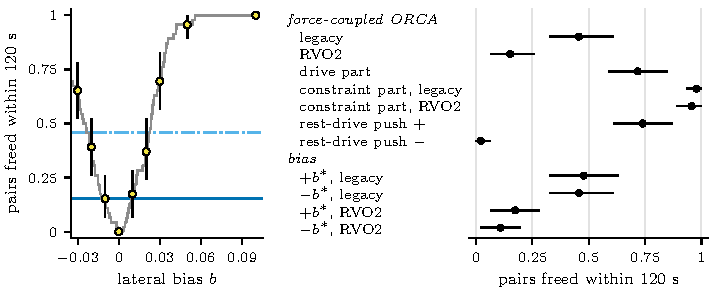
\includegraphics[width=\textwidth]{../figures/fig7_pair.pdf}
\caption{Pair standoffs freed within 120\,s against the lateral bias $b$ (left; grey steps, static threshold prediction; force-coupled ORCA, legacy dash-dot, RVO2 solid) and per perturbation (right), with 95\% bootstrap intervals over snapshots. Noise is not shown (Sect.~\ref{sec:pair}).}
\label{fig:pair}
\end{figure}
%
\subsubsection{Drive and Constraint Parts.}
Force-coupled ORCA frees \RzToneLegacyFreed\ of the \PairN\ standoffs [\RzToneLegacyLo, \RzToneLegacyHi] with the legacy solver and \RzToneRvoFreed\ [\RzToneRvoLo, \RzToneRvoHi] with the RVO2 solver (discordant \RzToneLegRvoA:\RzToneLegRvoB, McNemar $p=\RzToneLegRvoP$; Fig.~\ref{fig:pair}). Replays change no outcome with either solver (\TabThreePairRvoReplayDis\ and \TabThreePairPubReplayDis\ of \TabThreePairOrcaReplays). Quenches run on to 600\,s show that these counts are final: under no perturbation does a standoff free or come to rest after 120\,s, and the members of held standoffs move by at most \RzToneDispMax\,cm. The drive part alone frees \RzToneDriveFreed\ [\RzToneDriveLo, \RzToneDriveHi] and SFM \RzToneSfmFreed\ [0, \RzToneSfmHi]. The push frees \PairFrozenPlusFreed\ towards the door and \PairFrozenMinusFreed\ away. At rest the half-plane against the partner binds at all \RevAelevenPairBinds\ members, and the constraint part points laterally away from the partner with \RevAelevenRatioMin--\RevAelevenRatioMax\ of the magnitude of the drive part. This rest field is not a gradient (its Jacobian is not symmetric), and the stability argument of Sect.~\ref{sec:rest} does not cover force-coupled ORCA at the pair standoff. Alone, the constraint part frees \PairConsPubFreed\ standoffs (legacy) and \RzToneConsFreed\ [\RzToneConsLo, \RzToneConsHi] (RVO2). Each part alone thus frees most standoffs, the constraint part more than the drive part, yet together they free \RzToneRvoFreed: added to the drive part, the constraint part cancels the drive's lateral component towards the axis, and force-coupled ORCA frees fewer standoffs than the drive part alone ($p\PairDriveRvoPRel$). Of the \RevAelevenPairDisc\ standoffs that the drive part frees and force-coupled ORCA holds, the rest field accounts for \RevAelevenPairDiscStatic. The others, and the difference between the solvers, arise in motion, as the half-plane turns doorwards.

\subsubsection{Matched Lateral Bias.}
The matched bias $b^\ast$ is read off the thresholds $b_f$ of the same snapshots, so it is tuned in sample and reproduces each solver's freed fraction at $T=120$\,s by construction. Fitted on half the standoffs, it predicts force-coupled ORCA's freed fraction on the other half with median error $\RvAsixLegacyErrMedian$ (legacy) and $\RvAsixRvoErrMedian$ (RVO2). With the legacy solver $+b^\ast$ frees \PairBsPubFreed\ of the \PairN\ standoffs and with the RVO2 solver \PairBsRvoFreed; its replays change none (\TabThreePairBsPubReplayDis\ and \TabThreePairBsRvoReplayDis\ of \TabThreePairBsReplays).

With either solver equality of the bias and force-coupled ORCA is not rejected in freed fraction (difference \PscrPairPubDiff, Holm $p\RevAsevenPairPubFreedPHolmRel$ and $p\RevAsevenPairRvoFreedPHolmRel$; Table~\ref{tab:matched}) or in restricted mean time to free ($\PscrTimePairPubEff$\,s [$\PscrTimePairPubLo$, $\PscrTimePairPubHi$] legacy, $\PscrTimePairRvoEff$\,s [$\PscrTimePairRvoLo$, $\PscrTimePairRvoHi$] RVO2; Holm $p\RevAsevenPairPubTimePHolmRel$ for both). Equivalence within $\pm\RvAfiveMargin$ is not shown: the \PairN\ standoffs are too few (90\% interval [$\RvAfivePairLegacyDiffLoNinety$, $\RvAfivePairLegacyDiffHiNinety$] legacy). The freed sets overlap as much as independent sets would, with $\Omega=\RevAninePairPubJ$ against \RevAninePairPubEJ\ (legacy, $p\RevAninePairPubPRel$) and $\Omega=\RevAninePairRvoJ$ against \PscrPairRvoEJ\ (RVO2; $p\RevAninePairRvoPLeRel$ for an overlap this small or smaller).

Handedness separates the bias from force-coupled ORCA. The member below the door axis, which $b>0$ favours, exits first in all \PairBsPubHand\ standoffs that $+b^\ast$ frees with the legacy solver and all \TabThreePairRvoHand\ with the RVO2 solver. Under force-coupled ORCA it exits first in \PairPubLower\ of \PairPubFreed\ freed standoffs (legacy, Holm $p\RevAsevenPairPubHandPHolmRel$) and \TabThreePairRvoOrcaLower\ of \PairRvoFreed\ (RVO2, $p\RevAsevenPairRvoHandPHolmRel$). The reversed bias $-b^\ast$ frees \PairBsPubMinusFreed\ standoffs (legacy) and \PscrPairBsRvoMinusFreed\ (RVO2), with the member above the axis first in all of them.

\subsection{The ORCA Velocity Filter}\label{sec:velorca}
The ORCA velocity filter (Eq.~\eqref{eq:velorca}) frees no saved deadlock. At a snapshot no two agents are in contact, so every half-plane admits $\mathbf v=\mathbf 0$ with slack at least $(d_{ij}-r_{ij})/2\tau_h$; the filter returns $\mathbf v=\mathbf 0$, adding no rest drive. With either solver it frees \VelLoneRvoK\ of \VelLoneN\ lone-trap and \VelPairRvoK\ of \VelPairN\ pair quenches; its replays are identical. On the first \VelWholeN\ whole-run seeds (Table~\ref{tab:runsets}) \VelWholeK\ run completes under the filter and \VelWholeSfmK\ under SFM, against \VelWholeForceK\ under force-coupled ORCA (McNemar $p\VelWholeForcePRel$). All \VelWholeFail\ failures end at rest in states SFM also holds, so the filter acts at most while the crowd moves.

\subsection{Assigned Classes}\label{sec:classes}
The probe responses assign each perturbation to one class. Force-coupled ORCA frees deterministically at both rest states (identical RVO2 replays, a freed set that does not change with $\Delta t$, freeing under the push towards the door only); its drive part is an axial and its constraint part a lateral Reshape mechanism. Per-step noise frees with seeds that disagree and with an escape rate that falls as $\Delta t$ grows, as Eq.~\eqref{eq:ell} predicts with the measured slope ratio; it is a Heat mechanism. The lateral bias frees past $b_f$ with either sign, and the member on its favoured side exits first; it is a lateral Reshape mechanism. The ORCA velocity filter frees no snapshot and is at most a Prevent mechanism. The legacy solver adds replay sensitivity at the lone trap and, at the pair standoff, freed standoffs that vanish in the corrected implementation; it carries the defect flag.
